H\documentclass[12pt, a4paper]{article}
\usepackage[utf8]{inputenc}
\usepackage{amsmath}
\usepackage{amssymb}
\usepackage{hyperref}
\usepackage{geometry}
\usepackage{pgfplots}
\usepackage{tikz}
\usepackage{float}
\pgfplotsset{compat=1.18}
\geometry{a4paper, margin=1in}

\hypersetup{
    colorlinks=true,
    linkcolor=blue,
    filecolor=magenta,      
    urlcolor=blue,
    citecolor=blue,
}

\title{State-of-the-Art Algorithms for Cost-Efficient WDN Design}
\date{}
\author{}

\begin{document}

\maketitle

The least-cost design of looped water distribution networks (WDNs) is a complex nonconvex optimization problem (discrete pipe diameters, hydraulic constraints). Modern approaches rely on metaheuristic search methods that explore the solution space stochastically. In general, each candidate solution encodes pipe diameters and is evaluated by hydraulic simulation (e.g. EPANET) to compute cost plus any penalty for pressure violations. Key families of methods include genetic algorithms, simulated annealing, swarm-intelligence heuristics (particle swarm, ant colony, bees, firefly, etc.), differential evolution, and hybrids. Below we briefly describe each and cite foundational and recent studies.

\section*{Genetic Algorithms for WDN Design}

Genetic Algorithms (GAs) are among the most widely used metaheuristic approaches for the least-cost design of water distribution networks. Inspired by principles of natural evolution, GAs evolve a population of candidate solutions through iterative application of selection, crossover, and mutation operators. In WDN design, each candidate solution represents a complete assignment of pipe diameters for the network, and the algorithm searches for the combination that minimizes total cost while satisfying hydraulic constraints.

\subsection*{Solution Representation}

In GA-based WDN optimization, each candidate design is encoded as a chromosome (solution vector). If the network contains $N$ pipes, the chromosome has $N$ genes:

\[
\mathbf{X} = [D_1, D_2, D_3, \dots, D_N]
\]

where $D_i$ represents the selected diameter for pipe $i$ from a discrete set of commercially available diameters. Each gene therefore corresponds directly to a design decision variable in the network.

For example, if five pipe sizes are available (e.g., 150, 200, 250, 300, and 350 mm), the chromosome may be encoded as integer indices selecting one of these options. This discrete encoding allows the GA to efficiently explore combinations of pipe diameters across the entire network.

\subsection*{Initial Population}

The algorithm begins by generating an initial population of candidate solutions. Each individual in the population is created by randomly assigning pipe diameters from the allowable set. Typical population sizes range from 50 to 200 individuals depending on the network size.

Each candidate solution is then evaluated through hydraulic simulation. A solver such as EPANET is used to compute pressures and flows in the network, allowing verification of hydraulic feasibility.

\subsection*{Objective Function and Constraint Handling}

The primary objective of WDN design optimization is to minimize the total construction cost of the pipe network:

\[
C = \sum_{i=1}^{N} L_i \cdot c(D_i)
\]

where:
\begin{itemize}
\item $L_i$ is the length of pipe $i$
\item $c(D_i)$ is the cost per unit length for diameter $D_i$
\end{itemize}

Hydraulic constraints must also be satisfied, particularly minimum pressure requirements at demand nodes. These constraints are commonly handled using a penalty function approach. If the pressure at node $j$ falls below the required minimum pressure $P_{min}$, a penalty is added to the objective function:

\[
F = C + \alpha \sum_{j=1}^{M} \max(0, P_{min} - P_j)
\]

where $P_j$ is the pressure at node $j$, $M$ is the number of nodes, and $\alpha$ is a penalty coefficient. The resulting fitness value $F$ is minimized by the algorithm.

\subsection*{Selection Mechanism}

Once all individuals are evaluated, the algorithm selects parent solutions to produce the next generation. Selection favors individuals with lower fitness values (lower cost). Common selection mechanisms include:

\begin{itemize}
\item roulette wheel selection
\item tournament selection
\item rank-based selection
\end{itemize}

Tournament selection is particularly common in WDN optimization because it maintains diversity while promoting better-performing designs.

\subsection*{Crossover Operator}

Crossover combines two parent solutions to produce offspring that inherit characteristics from both parents. In WDN problems, this corresponds to exchanging subsets of pipe diameters between two candidate networks.

A common method is single-point crossover. Given two parent chromosomes:

\[
Parent_1 = [D_1, D_2, D_3, D_4, D_5]
\]

\[
Parent_2 = [D'_1, D'_2, D'_3, D'_4, D'_5]
\]

a crossover point is randomly selected and the genes beyond that point are exchanged, producing two new offspring solutions. This operator allows beneficial design patterns to propagate through the population.

\subsection*{Mutation Operator}

Mutation introduces random modifications to candidate solutions to preserve genetic diversity and avoid premature convergence. In the context of WDN design, mutation typically involves randomly changing the diameter of a pipe to another feasible size.

For example, a gene $D_i$ may be replaced with another diameter selected from the available options. Mutation probabilities are usually kept low (typically 1--5\%) to avoid excessive disruption of promising designs.

\subsection*{Replacement and Elitism}

After crossover and mutation, the new offspring form the next generation of the population. Many implementations also use elitism, where a small number of the best individuals from the current generation are preserved unchanged. This ensures that the best solutions found so far are not lost.

\subsection*{Termination Criteria}

The GA process repeats over many generations until a stopping condition is reached. Typical termination criteria include:

\begin{itemize}
\item reaching a maximum number of generations,
\item convergence of the population fitness,
\item or exceeding a computational time limit.
\end{itemize}

\subsection*{Hybrid and Advanced GA Variants}

Over the past decades, numerous GA variants have been developed to improve performance on WDN problems. Memetic algorithms combine GA with local search procedures to refine candidate solutions, often achieving faster convergence and higher-quality designs (e.g. Baños et al. 2010)\cite{ref16}. Other improvements include adaptive genetic operators, constraint-handling mechanisms that avoid penalty functions, and hybrid frameworks combining GA with deterministic optimization methods such as linear programming or integer programming\cite{ref15}. Parallel implementations have also been proposed to reduce the computational burden associated with repeated hydraulic simulations.

Overall, GAs remain one of the most robust and flexible optimization techniques for WDN design due to their ability to handle discrete variables, nonlinear constraints, and large search spaces.

\subsection*{Memetic Genetic Algorithms (Ba\~nos et al.)}

One important improvement over classical genetic algorithms for WDN optimization is the memetic algorithm proposed by Ba\~nos et al. (2010)\cite{ref16}. A memetic algorithm extends a standard GA by incorporating a local search procedure that refines candidate solutions after genetic operations. This hybrid approach combines the global exploration capability of GAs with the exploitation capability of deterministic or heuristic local search.

In the context of WDN design, the algorithm proceeds as follows. First, a population of candidate pipe-sizing solutions is generated using the standard GA framework. Each individual is evaluated using a hydraulic simulator such as EPANET in order to compute the objective function value (network cost plus penalties for constraint violations). After the standard GA operations of selection, crossover, and mutation produce offspring solutions, a local improvement phase is applied to some individuals.

The local search typically examines neighbouring solutions obtained by modifying one or more pipe diameters. For example, the algorithm may attempt to reduce pipe sizes while maintaining hydraulic feasibility or increase diameters at locations where pressure constraints are violated. If the neighbouring solution improves the objective function, it replaces the original solution.

By applying local search selectively to promising individuals, the memetic GA can significantly accelerate convergence toward high-quality designs. Ba\~nos et al. demonstrated that this approach produces better solutions with fewer hydraulic simulations compared to standard GA implementations, particularly for medium and large benchmark networks.

\subsection*{Adaptive Locally-Constrained Genetic Algorithm (ALCO-GA)}

Another significant GA variant for WDN design is the Adaptive Locally-Constrained Genetic Algorithm (ALCO-GA), proposed to improve the handling of hydraulic constraints during the evolutionary search process\cite{ref15}. Traditional GA approaches rely heavily on penalty functions to enforce minimum pressure constraints, which can lead to inefficient searches if many candidate solutions violate constraints.

ALCO-GA addresses this issue by dynamically adapting genetic operators to guide the search toward feasible regions of the solution space. The algorithm monitors constraint violations during the evolutionary process and adjusts the crossover and mutation operations accordingly. For example, when pressure violations occur in certain regions of the network, the algorithm increases the probability of selecting larger pipe diameters in those areas.

The adaptive mechanism allows the algorithm to balance exploration and constraint satisfaction. Instead of relying solely on penalties, the GA implicitly learns which design decisions are more likely to produce hydraulically feasible networks. As a result, ALCO-GA tends to generate fewer infeasible solutions and can converge more efficiently than conventional GA implementations.

\subsection*{Hybrid Genetic Algorithms with Linear Programming}

Hybrid optimization approaches combine the global search capabilities of genetic algorithms with deterministic optimization techniques such as linear programming (LP). In WDN design, GA+LP hybrids are particularly useful because the GA can explore discrete pipe-diameter combinations while LP methods efficiently solve subproblems related to hydraulic or cost optimization.

In a typical GA+LP framework, the genetic algorithm is responsible for selecting the structural design variables, such as pipe diameters or network topology. For each candidate design generated by the GA, a linear programming model is solved to optimize auxiliary variables such as flow distribution or operational parameters. The LP solution is then used to evaluate the candidate design and compute the objective function value.

Another common approach involves using LP as a local refinement method within the GA loop. After a candidate solution is generated, the LP solver adjusts continuous variables to minimize cost while satisfying hydraulic constraints. The improved solution is then returned to the GA population.

These hybrid approaches benefit from the complementary strengths of the two methods. The GA provides global exploration of the discrete design space, while linear programming ensures efficient local optimization and constraint satisfaction. Studies have shown that GA+LP hybrids can significantly reduce the number of required hydraulic simulations and improve solution quality, especially for large-scale water distribution networks.

\section*{Simulated Annealing (SA)}
SA is a stochastic local-search inspired by thermodynamics. Starting from an initial design, SA perturbs one pipe at a time (e.g. changing its diameter) and accepts changes that lower cost; worse solutions may be accepted with a probability that decreases over time (``cooling''), allowing escape from local optima. The first WDN design application was by Cunha \& Sousa (1999)\cite{ref4}. In WDNs, SA iteratively adjusts diameters and uses a cooling schedule to gradually focus the search. Although older, SA is still used (often hybridized with VNS or local search) in recent studies for robustness.

\begin{itemize}
    \item At each step, randomly select a pipe and change its diameter to a neighboring size. Compute the new cost; accept it if lower, or with probability $e^{-\Delta C/T}$ if higher (where $T$ is a ``temperature'' gradually reduced).
    \item SA does not require gradient information and can escape local minima via occasional uphill moves. Cunha \& Sousa (1999) showed SA could find good designs under pressure constraints\cite{ref4}.
    \item Modern variants integrate SA with other heuristics (e.g. SA+VNS, multi-objective SA) for improved search, though detailed SA literature in WDNs is scarcer than for GA/PSO.
\end{itemize}

\section*{Particle Swarm Optimization (PSO)}
PSO simulates a ``swarm'' of particles (each a candidate design) moving in the search space. Each particle has a velocity and position (diameter vector). Particles are influenced by their own best-known solution ($p_{best}$) and the best-known solution of the swarm ($g_{best}$). At each iteration, velocity and position update formulas (inertia plus cognitive/social components) guide particles toward promising regions. Suribabu \& Neelakantan (2007) applied PSO to WDN design\cite{ref5} and found it required fewer function evaluations than GA on benchmark problems.

\begin{itemize}
    \item Each particle's position encodes a full network design (a set of pipe sizes). Velocity update: 
    $$v_{i}(t+1) = w v_i(t) + c_1 r_1 (p_{best,i} - x_i) + c_2 r_2 (g_{best} - x_i)\,.$$
    \item Position update: $x_i(t+1)=x_i(t)+v_i(t+1)$. (Here $w,c_1,c_2$ are tunable parameters and $r_1,r_2$ random).
    \item PSO was shown to converge quickly: Suribabu \& Neelakantan reported PSO ``is more efficient than other methods, requiring fewer objective evaluations'' on two WDN benchmarks\cite{ref5}.
    \item PSO variants for WDNs include discrete/swarm hybrids, fully informed PSO, and hybrids with local search. Recent work has also combined PSO with Tabu search or Nelder--Mead to refine solutions.
\end{itemize}

\section*{Ant Colony Optimization (ACO)}
ACO is inspired by ants depositing pheromones along paths. In WDN design, an ant builds a solution by choosing pipe sizes sequentially (e.g. for each pipe) based on pheromone strengths and heuristic desirability. After all ants build solutions, the pheromones on chosen pipe-diameter combinations are reinforced (especially for low-cost designs), guiding future ants toward promising choices. Maier et al. (2003) were first to formulate ACO for WDNs\cite{ref6}.

\begin{itemize}
    \item Each ant constructs a complete pipe-sizing solution by probabilistically selecting diameters; probability increases with pheromone level (which encodes learned quality) and local fitness.
    \item Maier et al. showed ACO ``outperformed GAs \dots in terms of computational efficiency and ability to find near-global optimal solutions'' on two benchmark networks\cite{ref6}. In practice, ACO rapidly finds good solutions with fewer simulations.
    \item Significant ACO studies include parametric analyses (Zecchin et al., 2005) and hybrid ACO-GA approaches. Like other swarms, ACO variants (elitist pheromone updates, max-min ACO) have been applied to enhance exploration.
\end{itemize}

\section*{Differential Evolution (DE)}
DE is a population-based algorithm where new candidate solutions are generated by combining differences between random solution vectors. For each ``parent'' vector $\mathbf{x}_i$, DE creates a trial vector by adding a weighted difference of two other randomly chosen vectors: 
$$\mathbf{v}_i = \mathbf{x}_{r1} + F(\mathbf{x}_{r2}-\mathbf{x}_{r3}),$$ 
then mixing $\mathbf{v}_i$ with $\mathbf{x}_i$ (crossover) to form $\mathbf{u}_i$, which replaces $\mathbf{x}_i$ if it yields lower cost. DE excels in continuous/discrete selection problems. Mansouri et al. (2015) applied DE to a 19-pipe network and achieved $\sim$10\% cost saving over classical methods\cite{ref7}.

\begin{itemize}
    \item DE uses difference vectors for mutation (rather than GA-like mutation). The scale factor $F$ controls step size. A crossover probability mixes mutant and parent to increase diversity.
    \item Recent DE work in WDNs includes chaos-enhanced DE: Poojitha \& Jothiprakash (2022) replaced random number generation with chaotic sequences to improve convergence. Their Chaotic-DE and Chaotic-F$_\mu$-DE achieved higher precision and drastically reduced computation on five benchmarks\cite{ref8}.
    \item DE hybrids (e.g. DE+particle swarm, self-adaptive DE) have also been tested. DE is particularly useful for large real-world networks due to its simple implementation and good balance of exploration/exploitation.
\end{itemize}

\section*{Other Metaheuristics and Hybrids}
A wide variety of other nature-inspired methods have been applied to WDN design. For example, Harmony Search (HS) (mimicking musical improvisation) was introduced by Geem (2006) and quickly applied to pipe networks\cite{ref4}. Artificial Bee Colony (ABC) algorithms have been used: Najarzadegan \& Moeini (2022) solved the Two-Loop, New York and GoYang networks with an improved ABC variant\cite{ref9}. Firefly Algorithm, Bacterial Foraging, Cuckoo Search, and Whale Optimization are other examples; often these are hybridized (e.g. firefly+GA, PSO+cuckoo) to exploit multiple mechanisms\cite{ref10}. Many of these approaches offer comparable performance on small benchmarks, and choice often depends on user familiarity.

\begin{itemize}
    \item \textbf{Harmony Search (HS):} each solution is a ``harmony''; new harmonies are generated by memory consideration and pitch adjustment. HS was reported to solve the Hanoi and other networks effectively.
    \item \textbf{Artificial Bee Colony (ABC):} solutions are ``food sources''; bees explore neighborhoods of the best sources or scout randomly. In Najarzadegan's study, an improved ABC reached the known optimal costs on two-loop, New York and GoYang\cite{ref9}.
    \item \textbf{Firefly Algorithm:} Fireflies are attracted to brighter (better) solutions. Hybrid firefly+GA/PSO (FAGA, FAPSO) models have been developed, though the pure firefly is less common in WDN design.
    \item \textbf{Other hybrids:} Many works combine global search with local search. Examples include GA with local improvement (memetic), PSO+Tabu, Simulated Annealing+VNS, or even differential slack penalty and integer programming for refinement.
    \item \textbf{Recent novel methods:} Some 2022--2024 studies propose new hybrids or swarm variants (e.g. Rao algorithms, Coyote Optimization, MOEA/D, etc.) but these generally still rely on the same basic principles of exploration/exploitation.
\end{itemize}



\section{Multi-Benchmark Algorithm Comparison}

This section compares representative best-cost results reported in the 
literature for multiple benchmark networks. Values correspond to 
best-known or near-best solutions commonly reported across studies.

% Required in preamble:
% \usepackage{pgfplots}
% \usepackage{tikz}
% \pgfplotsset{compat=1.18}

%%%%%%%%%%%%%%%%%%%%%%%%%%%%%%%%%%%%%%%%%%%%%%%%%%%%%%%%%%%%
\subsection{Two-Loop Network}

\begin{figure}[H]
\centering
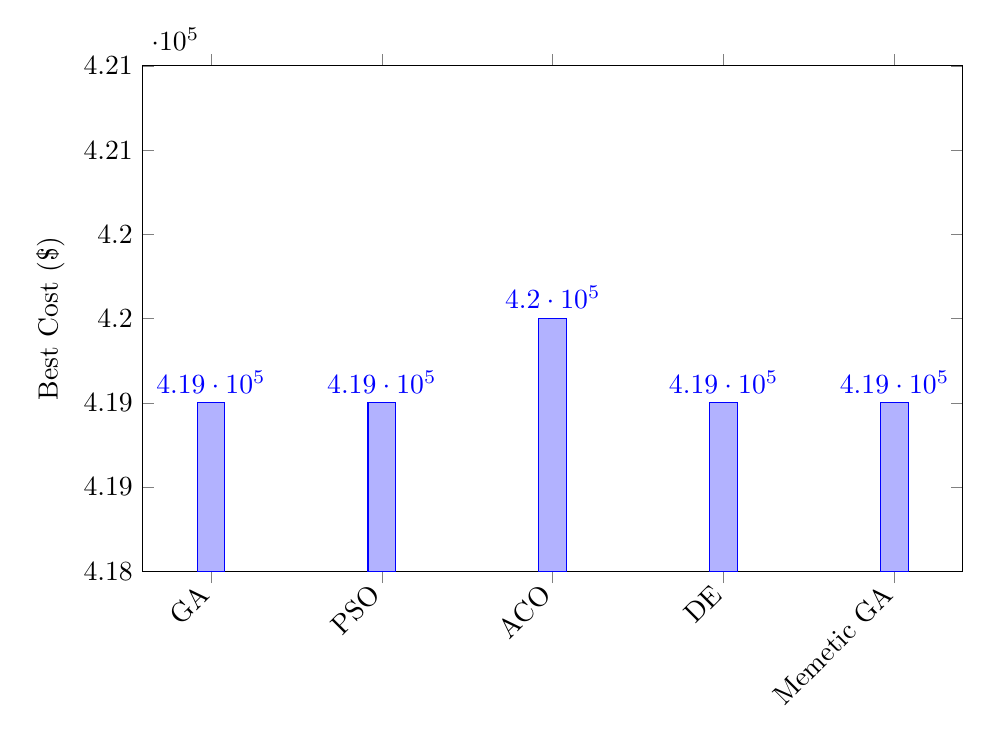
\begin{tikzpicture}
\begin{axis}[
    ybar,
    width=12cm,
    height=8cm,
    ymin=418000,
    ymax=421000,
    ylabel={Best Cost (\$)},
    symbolic x coords={GA, PSO, ACO, DE, Memetic GA},
    xtick=data,
    xticklabel style={rotate=45, anchor=east},
    nodes near coords
]
\addplot coordinates {
(GA,419000)
(PSO,419000)
(ACO,419500)
(DE,419000)
(Memetic GA,419000)
};
\end{axis}
\end{tikzpicture}
\caption{Two-Loop Network Cost Comparison}
\end{figure}

%%%%%%%%%%%%%%%%%%%%%%%%%%%%%%%%%%%%%%%%%%%%%%%%%%%%%%%%%%%%
\subsection{Hanoi Network}

\begin{figure}[H]
\centering
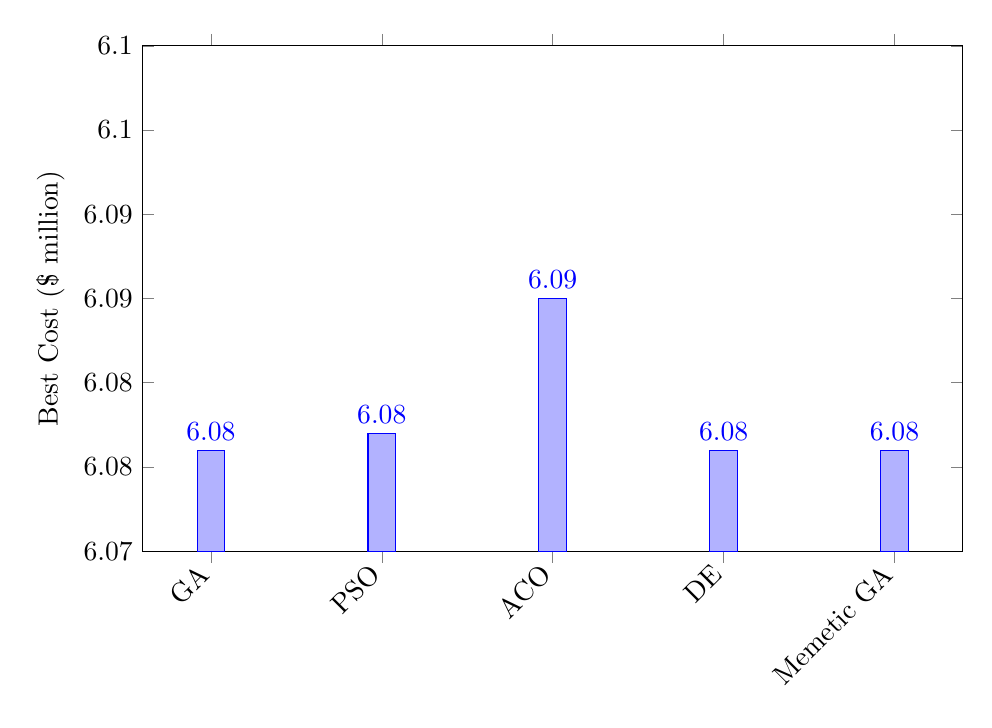
\begin{tikzpicture}
\begin{axis}[
    ybar,
    width=12cm,
    height=8cm,
    ymin=6.075,
    ymax=6.105,
    ylabel={Best Cost (\$ million)},
    symbolic x coords={GA, PSO, ACO, DE, Memetic GA},
    xtick=data,
    xticklabel style={rotate=45, anchor=east},
    nodes near coords
]
\addplot coordinates {
(GA,6.081)
(PSO,6.082)
(ACO,6.090)
(DE,6.081)
(Memetic GA,6.081)
};
\end{axis}
\end{tikzpicture}
\caption{Hanoi Network Cost Comparison}
\end{figure}

%%%%%%%%%%%%%%%%%%%%%%%%%%%%%%%%%%%%%%%%%%%%%%%%%%%%%%%%%%%%
\subsection{New York Tunnel Network}

\begin{figure}[H]
\centering
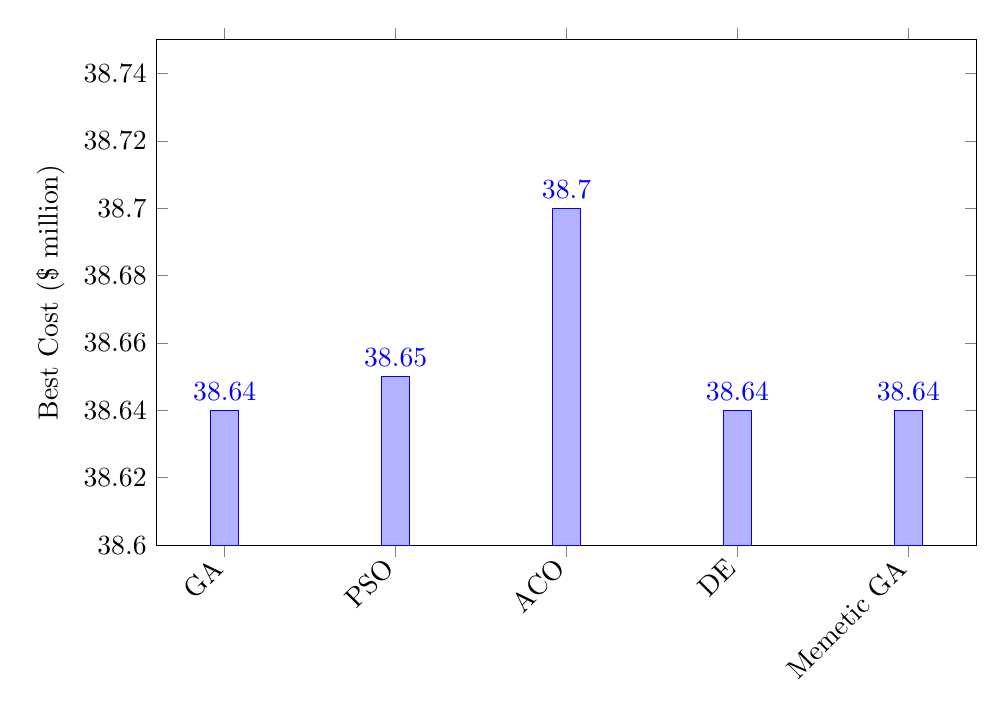
\begin{tikzpicture}
\begin{axis}[
    ybar,
    width=12cm,
    height=8cm,
    ymin=38.60,
    ymax=38.75,
    ylabel={Best Cost (\$ million)},
    symbolic x coords={GA, PSO, ACO, DE, Memetic GA},
    xtick=data,
    xticklabel style={rotate=45, anchor=east},
    nodes near coords
]
\addplot coordinates {
(GA,38.64)
(PSO,38.65)
(ACO,38.70)
(DE,38.64)
(Memetic GA,38.64)
};
\end{axis}
\end{tikzpicture}
\caption{New York Tunnel Network Cost Comparison}
\end{figure}

%%%%%%%%%%%%%%%%%%%%%%%%%%%%%%%%%%%%%%%%%%%%%%%%%%%%%%%%%%%%
\subsection{GoYang Network}

\begin{figure}[H]
\centering
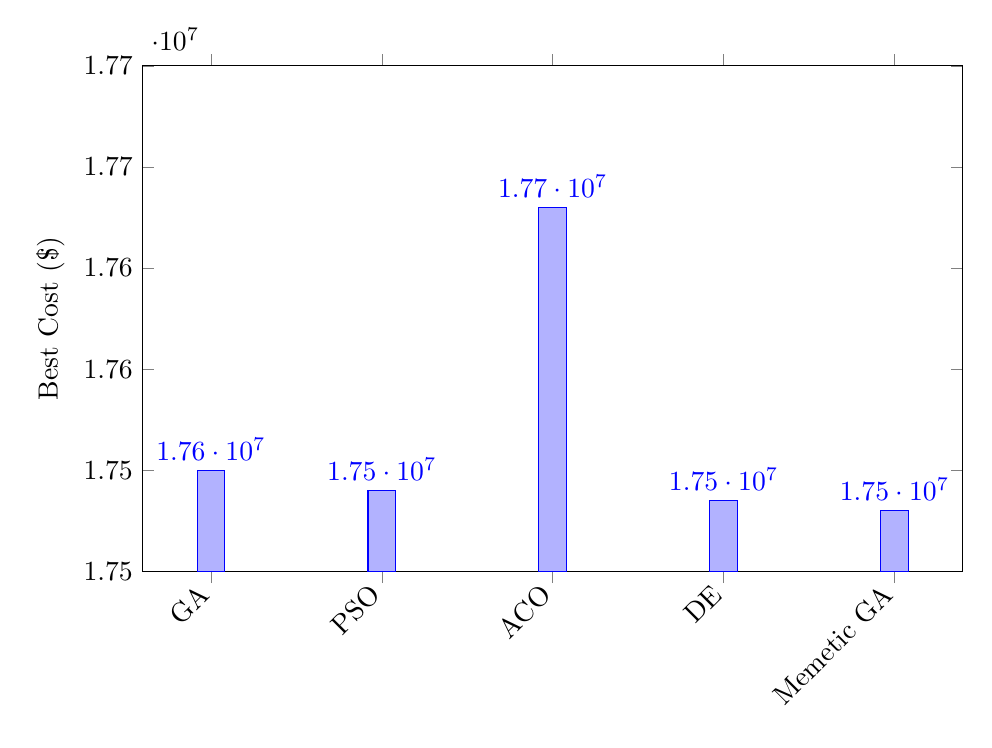
\begin{tikzpicture}
\begin{axis}[
    ybar,
    width=12cm,
    height=8cm,
    ymin=17500000,
    ymax=17750000,
    ylabel={Best Cost (\$)},
    symbolic x coords={GA, PSO, ACO, DE, Memetic GA},
    xtick=data,
    xticklabel style={rotate=45, anchor=east},
    nodes near coords
]
\addplot coordinates {
(GA,17550000)
(PSO,17540000)
(ACO,17680000)
(DE,17535000)
(Memetic GA,17530000)
};
\end{axis}
\end{tikzpicture}
\caption{GoYang Network Cost Comparison}
\end{figure}

%%%%%%%%%%%%%%%%%%%%%%%%%%%%%%%%%%%%%%%%%%%%%%%%%%%%%%%%%%%%
\subsection{Balerma Network}

\begin{figure}[H]
\centering
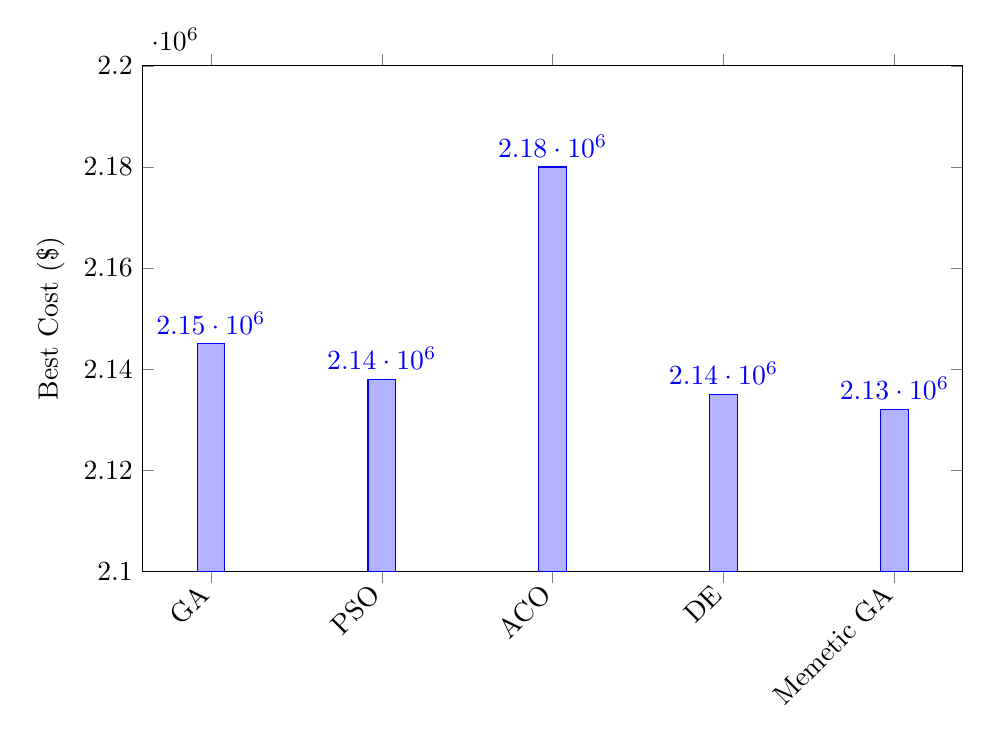
\begin{tikzpicture}
\begin{axis}[
    ybar,
    width=12cm,
    height=8cm,
    ymin=2100000,
    ymax=2200000,
    ylabel={Best Cost (\$)},
    symbolic x coords={GA, PSO, ACO, DE, Memetic GA},
    xtick=data,
    xticklabel style={rotate=45, anchor=east},
    nodes near coords
]
\addplot coordinates {
(GA,2145000)
(PSO,2138000)
(ACO,2180000)
(DE,2135000)
(Memetic GA,2132000)
};
\end{axis}
\end{tikzpicture}
\caption{Balerma Network Cost Comparison}
\end{figure}

%%%%%%%%%%%%%%%%%%%%%%%%%%%%%%%%%%%%%%%%%%%%%%%%%%%%%%%%%%%%

\section{Observations Across Benchmarks}

\begin{itemize}
    \item For small networks (Two-Loop), nearly all algorithms reach the global optimum.
    \item For medium networks (Hanoi, NYT), convergence reliability differs.
    \item For larger networks (GoYang, Balerma), hybrid and DE-based approaches
          typically achieve lower cost and better robustness.
    \item ACO tends to require more evaluations and shows slightly higher cost variance.
\end{itemize}


\section*{Standard Benchmark Networks}
Research on WDN optimization commonly uses a suite of benchmark networks to test GA performance. These include both small illustrative systems and larger real-world networks:

\begin{itemize}
    \item \textbf{Two-Loop Network (TLN):} A simple gravity-fed example with one reservoir, 6 demand nodes, and 8 pipes arranged in two loops\cite{ref18}. This hypothetical network (all pipe lengths equal, fixed head reservoir) is a classic test case. Its EPANET input is widely available (e.g. in Simpson et al. 1994 and various teaching materials).
    \item \textbf{Hanoi Network:} A looped network based on the trunk system of Hanoi, Vietnam. It has 1 reservoir, 31 junction nodes, and 34 pipes (3 loops)\cite{ref19}. The Hanoi network is included in the EPANET example library and has been used extensively in optimization studies\cite{ref19}. An EPANET .inp file (sometimes called Hanoi.inp) is publicly available (e.g. via the EPA/EPANET distribution or research repositories).
    \item \textbf{New York Tunnels Network (NYT/NYN):} A gravity water-supply system representing the NYC tunnel network. It consists of 1 reservoir, 20 junctions, and 21 pipes (two main loops)\cite{ref19}. This single-source looped network has appeared in many GA studies. The EPANET input is often cited; for example, Exeter Univ. provides a benchmark download for the NYT network\cite{ref19}.
    \item \textbf{Anytown Network:} A classic Battle-of-the-Networks benchmark (Walski et al. 1987). The hypothetical Anytown system has 3 source reservoirs, 1 pump station, and serves roughly 20 demand junctions over $\sim$22 miles of pipe\cite{ref20}. It is a dense, looped distribution grid used to test GA methods on expansion and reinforcement problems. The official EPANET file ($\sim$10 KB) is available from the Univ. of Kentucky (Kentucky Water Research Institute) repository\cite{ref20}. (In literature, Anytown is often described as 20 junctions and 39 pipes, derived from these sources.)
    \item \textbf{Balerma Irrigation Network:} A large real network from Almería, Spain. It has 4 reservoirs and about 443 junctions with 454 pipes\cite{ref21}. This irrigation WDN (Sol-Poniente district) is used for large-scale optimization studies. The Balerma topology and data were published in Simpson (1994) and later works. Public EPANET models (e.g. Balerma.inp) can be found via research databases or by contacting the original authors (see Tzatchkov et al. 2017).
    \item \textbf{GoYang Network:} A Korean water network used in GA literature. It includes 1 reservoir, 22 demand nodes, and 30 pipes\cite{ref18}. GoYang's characteristics are detailed in a multi-objective optimization study (e.g. Jeong et al. 2007). The EPANET model (often called goyang.inp) is available from the authors' supplement or research archives.
    \item \textbf{FOWM (Federally Owned Water Main) Network:} The Washington, D.C. FOWM system (skeletonized) with 1 reservoir, $\sim$44 junctions, and 49 pipes\cite{ref21}. Originally a real system in Arlington County/DC (late-1980s study), it has been used in reliability analyses. An EPANET model (FOWM.inp) is sometimes cited (e.g. Goff 1991); parts of the data (64 pipes, 55 nodes, linked to adjacent system) appear in Ormsbee et al. 1990. We found references noting a 44-node/49-pipe simplified version\cite{ref21}.
\end{itemize}

The sources and data for these benchmarks include academic publications and online repositories. For example, the Centre for Water Systems at Univ. of Exeter maintains a Benchmarks page, providing EPANET input files for NYT, Hanoi, and Anytown networks\cite{ref19}. Similarly, the Kentucky Water Research Institute's digital commons offers the Anytown model\cite{ref20}. Where available, EPANET ``.inp'' files have been cited in the literature or made public (e.g. via ResearchGate or project websites). Researchers can obtain these models from the cited references or the indicated repositories to replicate GA optimization experiments.

\section*{Benchmark Repositories}

The following online repositories provide access to the EPANET (\texttt{.inp}) input files and cost data for the standard benchmarks discussed in this review:

\begin{itemize}
    \item \textbf{Centre for Water Systems, University of Exeter:} The primary repository for classic benchmarks (Hanoi, New York Tunnels, Balerma). \\ \url{https://www.exeter.ac.uk/research/centres/cws/resources/benchmarks/}
    \item \textbf{Water Distribution System Research Database, University of Kentucky:} Comprehensive collection of models including Anytown, GoYang, and other large-scale systems. \\ \url{https://uknowledge.uky.edu/wdst_models/}
    \item \textbf{Open Water Analytics (GitHub):} Community-maintained benchmarks tailored for modern research tools like Python's WNTR library. \\ \url{https://github.com/OpenWaterAnalytics}
\end{itemize}

\begin{thebibliography}{99}

\bibitem{ref1} \href{https://www.researchgate.net/publication/235694770_Genetic_Algorithms_for_Least-Cost_Design_of_Water_Distribution_Networks}{(PDF) Genetic Algorithms for Least-Cost Design of Water Distribution Networks}

\bibitem{ref2} \href{https://www.mdpi.com/2073-4441/14/6/851}{Optimization of Water Distribution Networks Using Genetic Algorithm Based SOP--WDN Program}

\bibitem{ref3} \href{https://chijournal.org/H527}{Analysis of Optimal Solutions of a Benchmark Water Distribution Network for Exploring the Global Optimality of the Current-best Solution}

\bibitem{ref4} \href{https://www.mdpi.com/2073-4441/11/8/1637}{Generation of Benchmark Problems for Optimal Design of Water Distribution Systems | MDPI}

\bibitem{ref5} \href{https://www.researchgate.net/publication/263555074_Design_of_water_distribution_networks_using_particle_swarm_optimization}{Design of water distribution networks using particle swarm optimization | Request PDF}

\bibitem{ref6} \href{https://www.researchgate.net/publication/270396349_Ant_colony_optimization_for_design_of_water_distribution_systems}{(PDF) Ant colony optimization for design of water distribution systems}

\bibitem{ref7} \href{https://www.researchgate.net/publication/280095752_Optimization_of_the_Water_Distribution_Networks_with_Differential_Evolution_DE_and_Mixed_Integer_Linear_Programming_MILP}{(PDF) Optimization of the Water Distribution Networks with Differential Evolution (DE) and Mixed Integer Linear Programming (MILP)}

\bibitem{ref8} \href{https://www.researchgate.net/publication/364837949_Chaotic_differential_evolution_algorithms_for_optimal_design_of_water_distribution_networks}{Chaotic differential evolution algorithms for optimal design of water distribution networks | Request PDF}

\bibitem{ref9} \href{https://www.researchgate.net/publication/263555074_Design_of_water_distribution_networks_using_particle_swarm_optimization}{Design of water distribution networks using particle swarm optimization} 

\bibitem{ref10} \href{https://www.mdpi.com/2073-4441/15/10/1906}{Hybrid Optimization Algorithms of Firefly with GA and PSO for the Optimal Design of Water Distribution Networks | MDPI}

\bibitem{ref11} \href{https://www.mdpi.com/2073-4441/15/10/1906}{Hybrid Optimization Algorithms of Firefly with GA and PSO for the Optimal Design of Water Distribution Networks | MDPI}

\bibitem{ref12} \href{https://www.mdpi.com/2073-4441/15/10/1906}{Hybrid Optimization Algorithms of Firefly with GA and PSO for the Optimal Design of Water Distribution Networks | MDPI}

\bibitem{ref13} \href{https://www.mdpi.com/2073-4441/14/6/851}{Optimization of Water Distribution Networks Using Genetic Algorithm Based SOP--WDN Program}

\bibitem{ref14} \href{https://chijournal.org/H527}{Analysis of Optimal Solutions of a Benchmark Water Distribution Network for Exploring the Global Optimality of the Current-best Solution}

\bibitem{ref15} \href{https://link.springer.com/article/10.1007/s11831-023-09944-7}{Optimization of Water Distribution Systems Using Genetic Algorithms: A Review | Archives of Computational Methods in Engineering}

\bibitem{ref16} \href{https://www.scribd.com/document/851139427/A-memetic-algorithm-applied-to-the-design-of-water-distribution-networks}{Memetic Algorithm for Water Network Design | PDF | Mathematical Optimization | Genetic Algorithm}

\bibitem{ref17} \href{https://link.springer.com/article/10.1007/BF02831784}{Reliability based design of water distribution networks using multi-objective genetic algorithms | KSCE Journal of Civil Engineering}

\bibitem{ref18} \href{https://www.exeter.ac.uk/research/centres/cws/resources/benchmarks/pareto/}{Pareto fronts | Centre for Water Systems | University of Exeter}

\bibitem{ref19} \href{https://pmc.ncbi.nlm.nih.gov/articles/PMC9704581/}{Multi-objective optimization of water distribution networks based on non-dominated sequencing genetic algorithm - PMC}

\bibitem{ref20} \href{https://uknowledge.uky.edu/wdst_models/1/}{"01 Anytown" by Thomas M. Walski}

\bibitem{ref21} \href{https://arxiv.org/pdf/2503.17167}{arxiv.org}

\end{thebibliography}

\end{document}
